\documentclass[]{article}
\usepackage{float}
\usepackage{graphicx}

\title{Two Class PCA Analysis Report}
\author{}
\date{\today}

\begin{document}

\begin{titlepage}
    \maketitle
    \section*{Warnings}
    \section*{Data Summary}
\end{titlepage}

\section*{Principal Component Analysis (PCA) Summary}
    PCA analysis is performed using \texttt{sklearn} package version 1.1.2. \\
    Data scaling = \textbf{Standard}

    \begin{figure}[h!]
    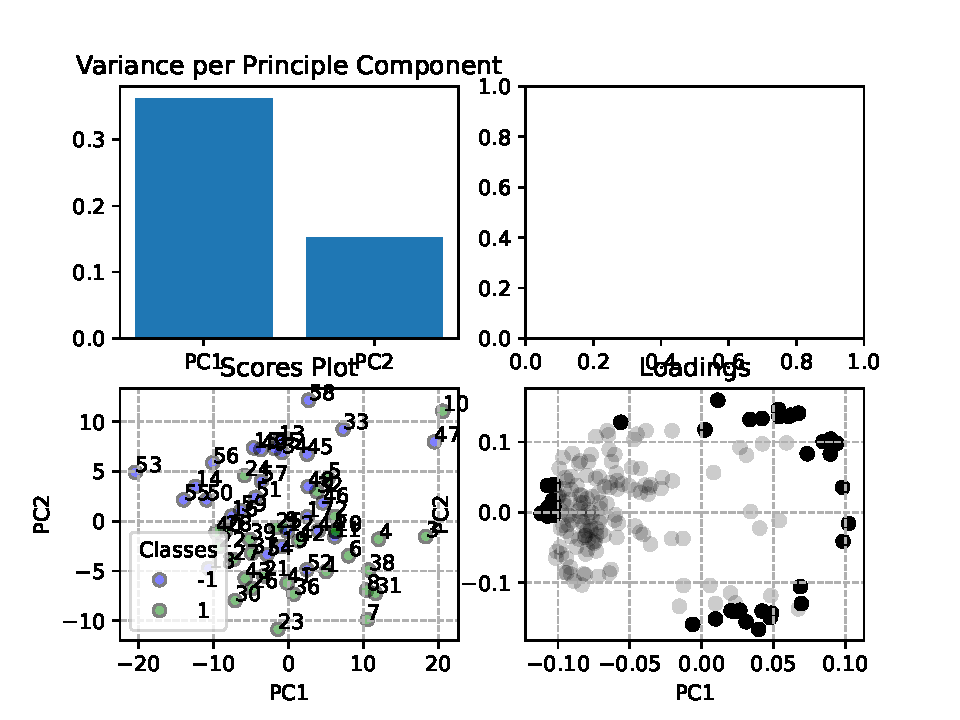
\includegraphics{summary_figs.pdf}
    \end{figure}

A table:
\begin{tabular}{ c | c | c | c }
    0 & 1 & 2 & 3\\
    4 & 5 & 6 & 7\\
    8 & 9 & 10 & 11\\
    12 & 13 & 14 & 15
\end{tabular}






\end{document}